% !TEX program = pdflatex
% ---------------------------------------------------------------------------
% Redundancy, not skill: separating near-duplicate leakage from training
% volume in high-entropy-alloy phase prediction
%
% Submission-ready source. Compile with pdflatex twice (for \ref) or use
% latexmk -pdf. Figures are expected in ./figures/.
% ---------------------------------------------------------------------------
\documentclass[11pt]{article}

\usepackage[T1]{fontenc}
\usepackage[utf8]{inputenc}
\usepackage[margin=1in]{geometry}
\usepackage{graphicx}
\usepackage{booktabs}
\usepackage{amsmath}
\usepackage{siunitx}
\usepackage[hidelinks]{hyperref}
\usepackage{authblk}

\graphicspath{{figures/}}

\title{\bfseries Redundancy, not skill: separating near-duplicate leakage\\ from training volume in high-entropy-alloy phase prediction}

\author[1]{[YOUR FULL NAME]}
\affil[1]{[SCHOOL NAME], Beijing, China}
\date{11 September 2026 \quad\textbar\quad preprint v1}

\begin{document}
\maketitle

\begin{abstract}
\noindent
Machine-learning models for high-entropy-alloy (HEA) phase prediction are routinely reported at \SI{85}{\percent}--\SI{95}{\percent} accuracy from randomly split data, even though published alloy datasets contain many compositions that differ only in stoichiometry. Removing such redundancy is known to cost accuracy, but published numbers conflate two things: losing redundant samples, and simply having less training data. I separate them.

Using 1{,}103 experimentally reported alloys (350 solid-solution, 753 not), I first confirm the redundancy is severe: the alloys occupy only 449 distinct element sets, \SI{74.9}{\percent} share a chemical system with another record, and 59 compositions are exact duplicates. I then run a size-matched exclusion sweep. For a radius $\tau$ in mole-fraction $L_1$ space, I train one model on all training alloys whose distance to the nearest test alloy is at least $\tau$, and a second model on a random subsample of the full pool of identical size. Both see the same number of examples; only the first is free of test-adjacent redundancy.

Gradient-boosted trees lose 0.198 balanced accuracy when \SI{62}{\percent} of the training set is removed by this filter. Of that loss, only 0.047 comes from the smaller training set; the remaining \textbf{0.151 (\SI{76}{\percent}) is what redundant, test-adjacent alloys were buying}. A $k$-NN classifier shows the same pattern (0.134 of 0.183, \SI{73}{\percent}), while a regularised logistic regression is essentially unaffected (0.032 of 0.044, not distinguishable from zero). The effect grows monotonically with $\tau$ and, importantly, is not driven by strict near-duplicates: excluding only the closest 0.05 $L_1$ shell changes boosted-tree accuracy by 0.010. The inflation lives in the 0.10--0.35 band --- same chemical system, nearby stoichiometry. Reported random-split accuracy for high-capacity models on this dataset is therefore overstated by roughly 0.08--0.15 balanced accuracy, and the overstatement tracks model capacity rather than feature choice.
\end{abstract}

\section{Why this needed doing}

A typical HEA machine-learning paper collects compositions and phase labels from the literature, computes empirical descriptors such as $\delta$, $\Delta H_{\mathrm{mix}}$, $\Omega$ and VEC, trains a classifier, and reports accuracy on a random test split. Numbers between 0.85 and 0.95 are common.

Experimental HEA records are not independent draws. Within one chemical system --- say Al--Co--Cr--Fe--Ni --- the literature contains dozens of alloys that differ only in how much of each element is present. A random split puts some of them in training and some in test. A flexible model can then answer many test questions by recalling a near-identical training alloy, which is memorisation rather than generalisation.

Leakage of this kind is well documented as a general phenomenon, including a dedicated data-splitting method for the life sciences \cite{datasail} and a broad review of leakage in machine-learning-based science \cite{kapoor}. I do not claim to discover it. What is missing for HEA specifically is a \emph{controlled} number: how much of the reported accuracy is redundancy, how much is just the smaller training set that a stricter split forces on you, and whether the split depends on model capacity. Without that separation, a reader cannot tell whether a reported 0.86 means ``the model generalises'' or ``the model remembered''.

Three questions: \textbf{Q1} how redundant is a standard open HEA dataset; \textbf{Q2} once redundancy is removed at fixed training size, how much accuracy disappears, and does that depend on model capacity; \textbf{Q3} where in composition space does the effect come from --- exact duplicates, or the broader same-system neighbourhood.

\section{Data}

Source: \emph{Materials for Design Open Repository. High Entropy Alloys}, Zenodo record 6403257 \cite{zenodo}, licence CC-BY-4.0. The raw workbook was downloaded once and never modified.

The label of interest is \texttt{S\_Phase}, recording phase constitution as SS (solid solution), SS+IM, IM (intermetallic) or AM (amorphous). Fourteen unlabelled records were dropped, leaving 1{,}103. The task is binarised: SS versus everything else, giving 350 positives and a base rate of \SI{31.7}{\percent}. A model that always answers ``not SS'' therefore scores 0.683 raw accuracy; every result below uses balanced accuracy, for which that baseline is 0.500.

Features are 78 elemental mole fractions plus nine design descriptors ($\delta$, $\Delta H_{\mathrm{mix}}$, $S_{\mathrm{id}}$, $\Omega$, VEC, $\sigma_{\mathrm{VEC}}$, $\Delta\chi$, $\chi$, $T_m$). $\Omega$ was recomputed from the Yang \& Zhang definition, $\Omega = T_m \Delta S_{\mathrm{mix}} / |\Delta H_{\mathrm{mix}}|$ \cite{yang}, rather than taken from the spreadsheet.

\begin{figure}[t]
\centering
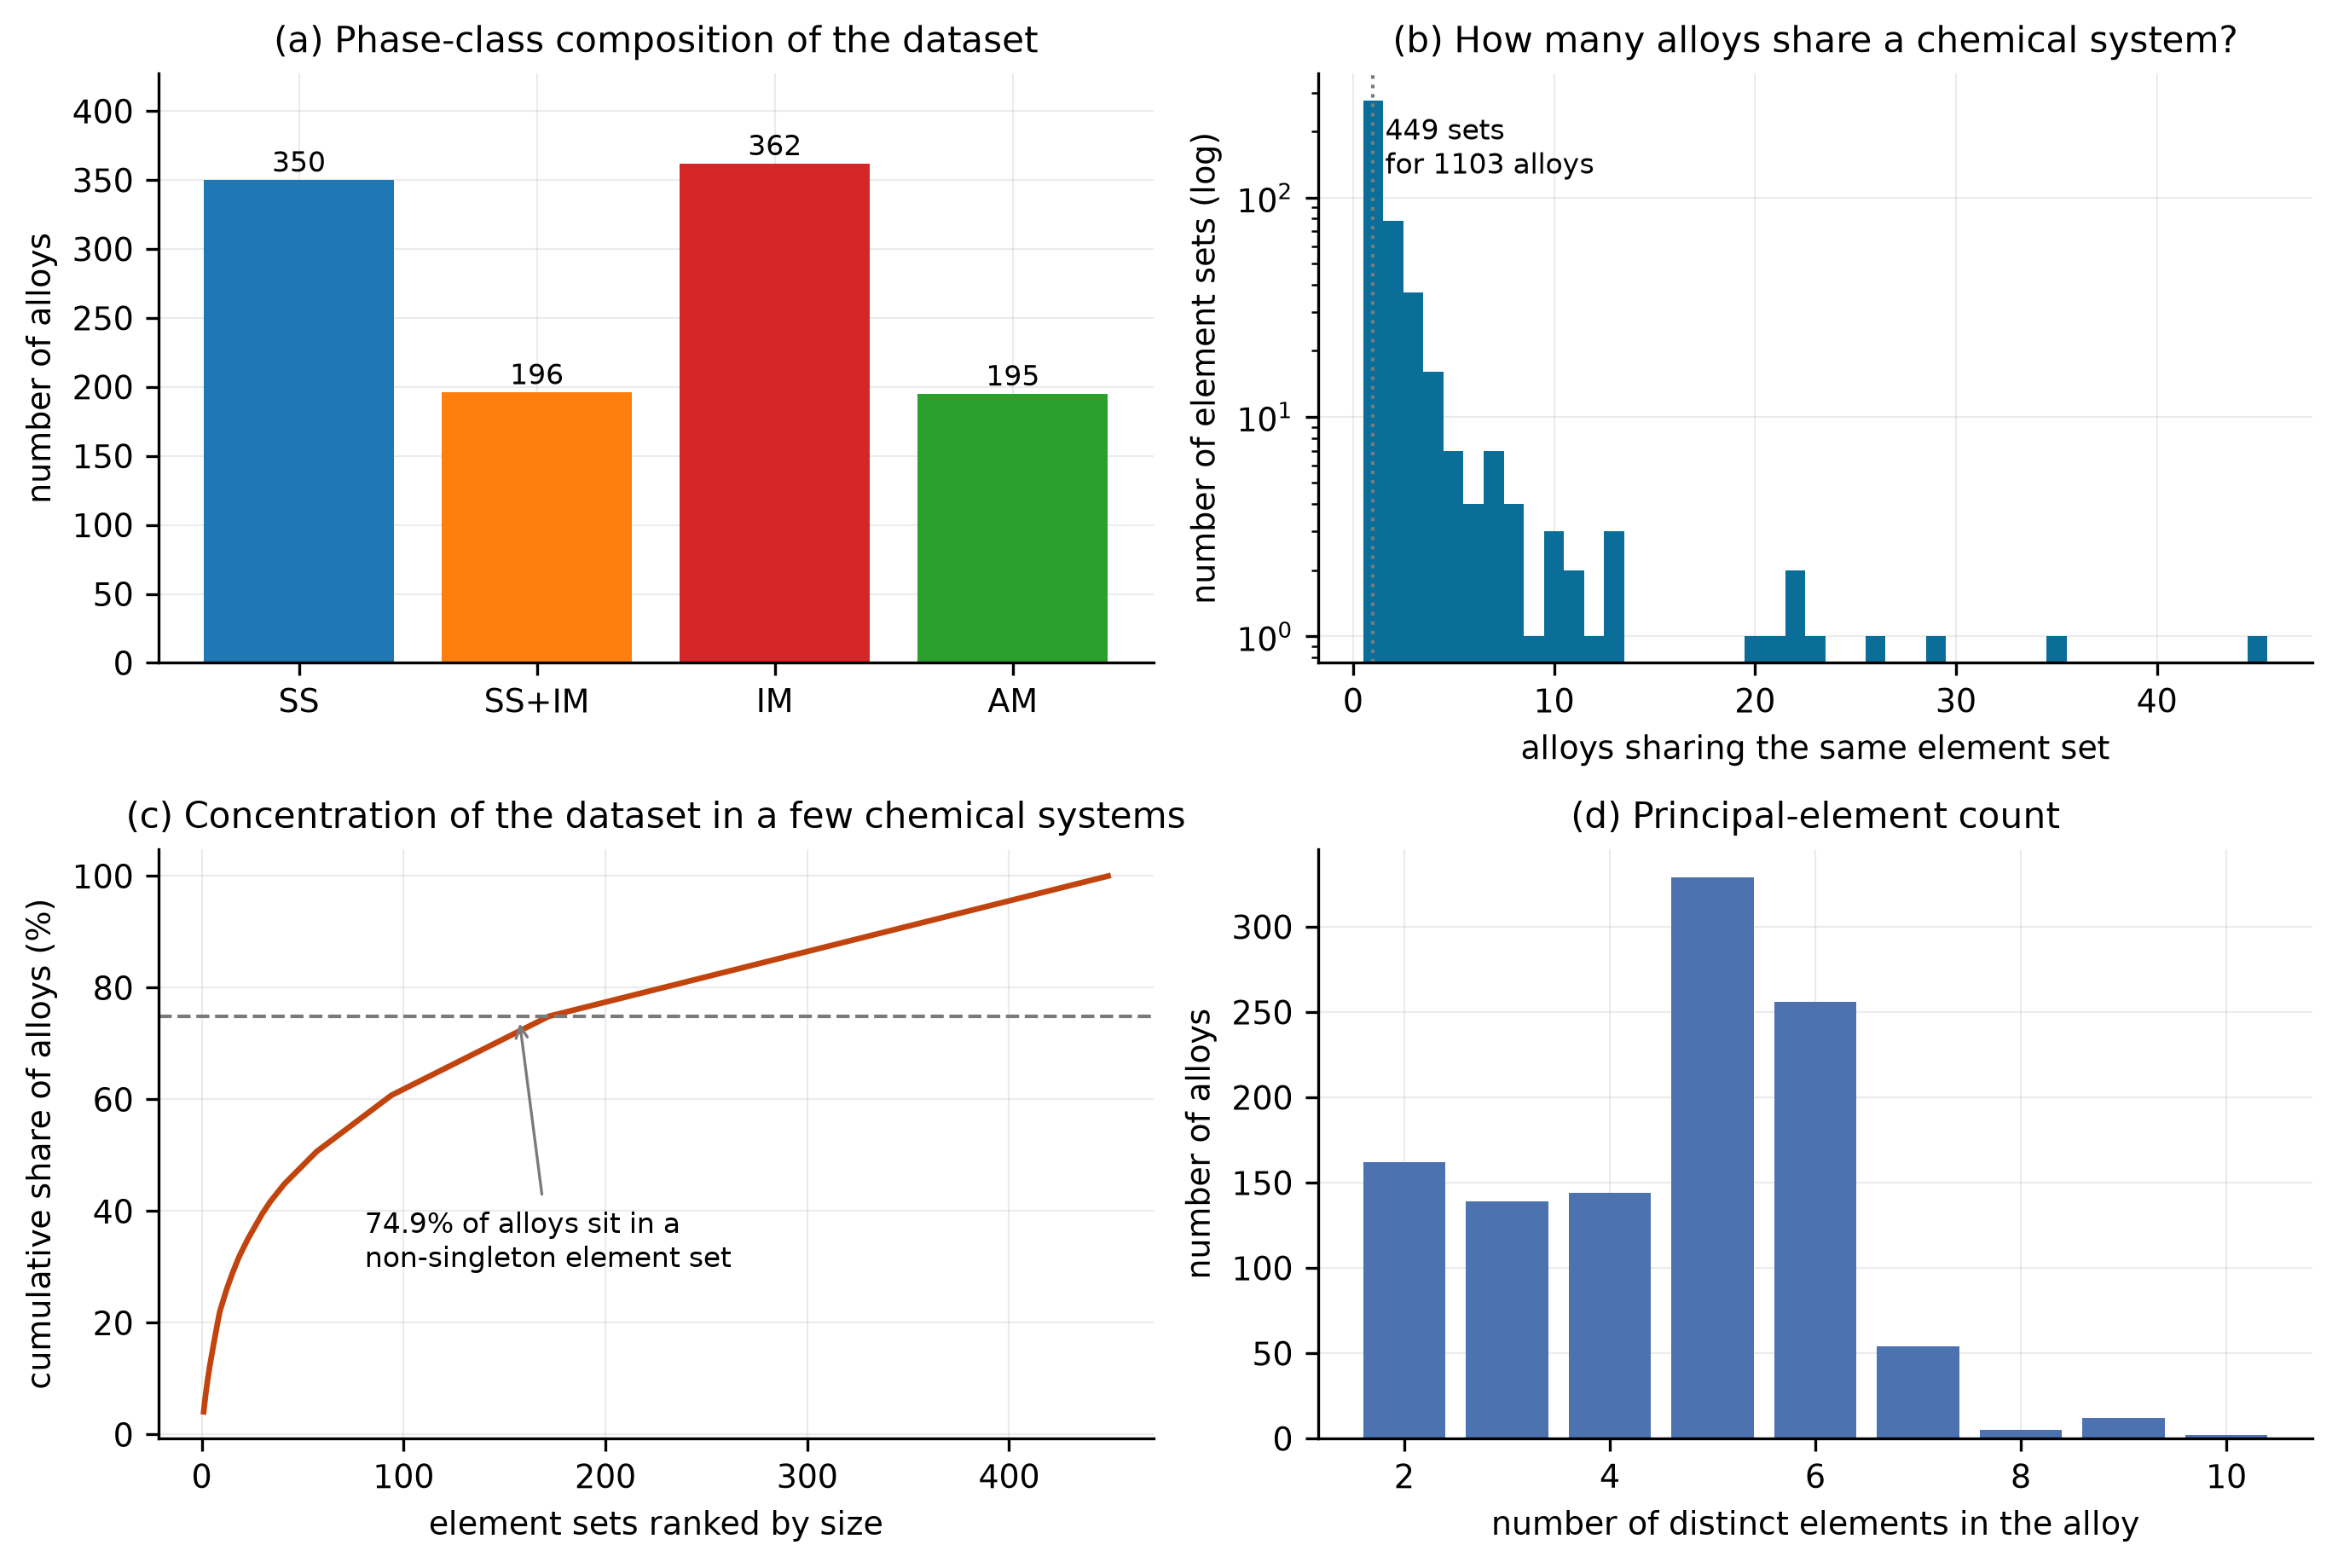
\includegraphics[width=\textwidth]{fig1_dataset_structure.png}
\caption{Redundancy structure of the dataset. Left: distribution of element-set sizes. Right: how many alloys share a chemical system.}
\label{fig:structure}
\end{figure}

\begin{table}[t]
\centering
\caption{Redundancy in the source dataset.}
\label{tab:redundancy}
\begin{tabular}{lr}
\toprule
Property & Value \\
\midrule
Labelled alloys & 1{,}103 \\
Solid-solution (positive class) & 350 (\SI{31.7}{\percent}) \\
Distinct element sets & 449 \\
Alloys in a shared chemical system & \SI{74.9}{\percent} \\
Largest single system & 45 alloys \\
Exact duplicate compositions & 59 \\
Elements appearing at least once & 57 \\
\bottomrule
\end{tabular}
\end{table}

The average chemical system holds 2.5 alloys, but the distribution is heavy-tailed: a few popular systems (Al--Co--Cr--Fe--Ni and its subsets, refractory Mo--Nb--Ta--V--W, the Ti--Zr--Hf family) supply a large fraction of the dataset. A random split of such a table is not a random split of chemical space.

\section{Methods}

\subsection{Models}

Three families spanning a wide capacity range.

\begin{itemize}
\item \textbf{Logistic regression} --- median imputation, standardisation, $L_2$ penalty ($C=1$), balanced class weights. Low capacity, strongly regularised.
\item \textbf{Histogram gradient-boosted trees} --- 150 iterations, learning rate 0.08, 15 leaves, $L_2 = 1.0$. High capacity.
\item \textbf{$k$-NN} --- $k=5$, distance weighting, cityblock metric on standardised features. Pure instance-based memory; included because if leakage is memorisation, this model should show it most clearly.
\end{itemize}

\subsection{Evaluation protocols}

\begin{enumerate}
\item \textbf{Random stratified CV} (5-fold, 3 repeats).
\item \textbf{Chemical-system-grouped CV} --- \texttt{StratifiedGroupKFold} with the element set as the group, so no system spans the split.
\item \textbf{Controlled paired experiment} --- a fixed \SI{20}{\percent} stratified test set. \texttt{TrainA\_matched} is the full training pool randomly subsampled; \texttt{TrainB\_disjoint} contains only alloys sharing no element set with any test alloy, subsampled to the same size. Same test set, same training size, 10 splits, Wilcoxon signed-rank test. The disjoint pool retains \SI{50.6}{\percent} of the full pool before matching.
\item \textbf{Near-duplicate exclusion sweep} (new; the core of this paper), described below.
\item \textbf{Leave-one-element-out} --- 18 frequent elements; train without element $X$, test only on alloys containing $X$.
\end{enumerate}

Metrics are balanced accuracy, MCC and ROC-AUC. Confidence intervals come from 2{,}000-resample bootstrap over test alloys. All seeds are fixed in the scripts.

\subsection{The exclusion sweep}

Protocols 1--3 show \emph{that} redundancy matters but not \emph{how much of the drop is redundancy}. Protocol 4 does.

Fix the test set $T$. For a radius $\tau$, compute for every training-pool alloy its $L_1$ distance, in mole-fraction space, to the nearest alloy in $T$. Then build two training sets of identical size $n$:

\begin{itemize}
\item \textbf{excluded$(\tau)$} --- the alloys with distance $\ge \tau$. Every test-adjacent neighbour has been physically removed.
\item \textbf{matched$(\tau)$} --- a uniformly random subsample of the \emph{whole} pool, of the same size $n$. Near-duplicates are still inside, but the training volume is identical.
\end{itemize}

Train the same model on each and score both on the same $T$. Define
\begin{equation}
\Delta(\tau) = \mathrm{balAcc}\big(\mathrm{matched}(\tau)\big) - \mathrm{balAcc}\big(\mathrm{excluded}(\tau)\big).
\end{equation}
Because the two training sets are the same size, the difference cannot be attributed to data volume. It is the accuracy that test-adjacent redundancy was supplying. Sweeping $\tau$ traces how that contribution is distributed across composition space: small $\tau$ isolates exact and near-exact duplicates, large $\tau$ reaches the whole same-system neighbourhood.

Seven radii were used, $\tau \in \{0, 0.02, 0.05, 0.08, 0.12, 0.20, 0.35\}$, over three splits. At $\tau = 0$ the two sets coincide by construction, which serves as a correctness check.

\section{Results}

\subsection{What the classical criteria are actually worth}

\begin{table}[t]
\centering
\caption{Classical phase-formation criteria evaluated on all 1{,}103 alloys.}
\label{tab:criteria}
\small
\begin{tabular}{lccccc}
\toprule
Criterion & Bal.\ acc. & \SI{95}{\percent} CI & Sens. & Spec. & MCC \\
\midrule
Always ``not SS''            & 0.500 & [0.500, 0.500] & 0.000 & 1.000 & 0.000 \\
$\delta \le \SI{6.6}{\percent}$ & 0.716 & [0.690, 0.740] & 0.860 & 0.571 & 0.405 \\
$-15 \le \Delta H_{\mathrm{mix}} \le 5$ & 0.689 & [0.663, 0.714] & 0.874 & 0.505 & 0.363 \\
$\Omega \ge 1.1$             & 0.714 & [0.692, 0.736] & 0.943 & 0.486 & 0.419 \\
$3 \le \mathrm{VEC} \le 8$   & 0.479 & [0.453, 0.504] & 0.774 & 0.183 & $-0.050$ \\
$\Delta\chi \le 0.3$         & 0.533 & [0.518, 0.548] & 0.966 & 0.101 & 0.114 \\
$\delta$ and $\Delta H_{\mathrm{mix}}$ & 0.731 & [0.704, 0.757] & 0.797 & 0.665 & 0.431 \\
$\delta + \Delta H_{\mathrm{mix}} + \Omega$ & \textbf{0.753} & [0.725, 0.779] & 0.786 & 0.720 & 0.474 \\
$\delta + \Delta H_{\mathrm{mix}} + \Omega + \mathrm{VEC}$ & 0.678 & [0.649, 0.708] & 0.569 & 0.788 & 0.354 \\
\bottomrule
\end{tabular}
\end{table}

The conjunction of $\delta$, $\Delta H_{\mathrm{mix}}$ and $\Omega$ reaches 0.753, the best of the classical rules. Adding VEC \emph{hurts} (0.678), because the VEC window is a poor discriminator for the SS-versus-not question --- it was designed for a different question, which lattice forms.

That distinction matters. Restricting attention to the 220 alloys whose phase is purely FCC or purely BCC, and applying the rule $\mathrm{VEC} \ge 8 \rightarrow$ FCC, $\mathrm{VEC} \le 6.87 \rightarrow$ BCC \cite{guo2011}, leaves 163 decidable cases (\SI{74.1}{\percent} coverage) and gets \textbf{all 163 right}. ``Does a solid solution form'' and ``which lattice does it adopt'' are therefore problems of very different difficulty; VEC answers the second well and is near-useless for the first.

\begin{table}[t]
\centering
\caption{Single-descriptor ceiling after cross-validated threshold tuning.}
\label{tab:single}
\begin{tabular}{llc}
\toprule
Descriptor & Direction & CV balanced accuracy \\
\midrule
$\Omega$      & higher $\rightarrow$ SS & $\mathbf{0.742 \pm 0.029}$ \\
$S_{\mathrm{id}}$ & higher $\rightarrow$ SS & $0.730 \pm 0.020$ \\
$\delta$      & lower $\rightarrow$ SS  & $0.728 \pm 0.021$ \\
$\Delta H_{\mathrm{mix}}$ & higher $\rightarrow$ SS & $0.684 \pm 0.025$ \\
$\Delta\chi$  & lower $\rightarrow$ SS  & $0.677 \pm 0.023$ \\
$T_m$         & higher $\rightarrow$ SS & $0.628 \pm 0.024$ \\
$\sigma_{\mathrm{VEC}}$ & lower $\rightarrow$ SS & $0.609 \pm 0.022$ \\
VEC           & lower $\rightarrow$ SS  & $0.513 \pm 0.024$ \\
\bottomrule
\end{tabular}
\end{table}

Even with the threshold chosen optimally by cross-validation, no single descriptor beats 0.742, and the classical three-rule conjunction matches that. Any model claiming 0.90+ on this task is doing something the descriptors cannot do on their own --- exactly the situation in which it is worth asking what it is doing.

\subsection{Random versus grouped cross-validation}

\begin{table}[t]
\centering
\caption{The same models and data under two splitting protocols.}
\label{tab:cv}
\begin{tabular}{llccc}
\toprule
Features & Model & Random stratified & System-grouped & Difference \\
\midrule
Composition only          & logreg & 0.787 & 0.730 & $+0.057$ \\
Composition only          & hgb    & 0.837 & 0.760 & $+0.077$ \\
9 descriptors only        & logreg & 0.798 & 0.796 & $+0.002$ \\
9 descriptors only        & hgb    & 0.850 & 0.763 & $+0.087$ \\
Composition + descriptors & logreg & 0.807 & 0.769 & $+0.038$ \\
Composition + descriptors & hgb    & 0.859 & 0.776 & $+0.083$ \\
\bottomrule
\end{tabular}
\end{table}

The boosted model loses 0.077--0.087 whatever features it is given, including when it sees \emph{only} the nine aggregate descriptors and no composition at all. The logistic regression barely moves on descriptors only ($+0.002$) but loses 0.057 on raw composition. Grouping hurts the low-capacity model only when it is handed the input that lets it identify the chemical system directly.

\subsection{Controlled paired comparison}

\begin{table}[t]
\centering
\caption{Controlled paired experiment: fixed test set, matched training size, 10 splits.}
\label{tab:paired}
\small
\begin{tabular}{llcccl}
\toprule
Features & Model & TrainA\_matched & TrainB\_disjoint & $\Delta$ & \SI{95}{\percent} CI \\
\midrule
Composition only          & hgb    & 0.787 & 0.638 & $+0.150$ & $[+0.106, +0.230]$ \\
Composition + descriptors & hgb    & 0.829 & 0.696 & $+0.133$ & $[+0.063, +0.196]$ \\
9 descriptors only        & hgb    & 0.806 & 0.690 & $+0.116$ & $[+0.067, +0.155]$ \\
Composition only          & logreg & 0.774 & 0.721 & $+0.053$ & $[+0.025, +0.090]$ \\
Composition + descriptors & logreg & 0.807 & 0.784 & $+0.023$ & $[-0.008, +0.055]$ \\
9 descriptors only        & logreg & 0.803 & 0.783 & $+0.021$ & $[-0.010, +0.049]$ \\
\bottomrule
\end{tabular}
\end{table}

All Wilcoxon $p \le 2.7\times10^{-2}$ except the logistic-regression composition+descriptor case, whose CI includes zero. For boosted trees, at identical training size and identical test set, chemical-system disjointness alone is worth $+0.133$ balanced accuracy.

Note that the descriptors-only boosted model still gains $+0.116$. The nine descriptors are deterministic functions of composition, so this is not evidence that the effect is about features; the effect travels with the sample, not with the representation.

\subsection{Separating redundancy from training volume}

\begin{figure}[t]
\centering
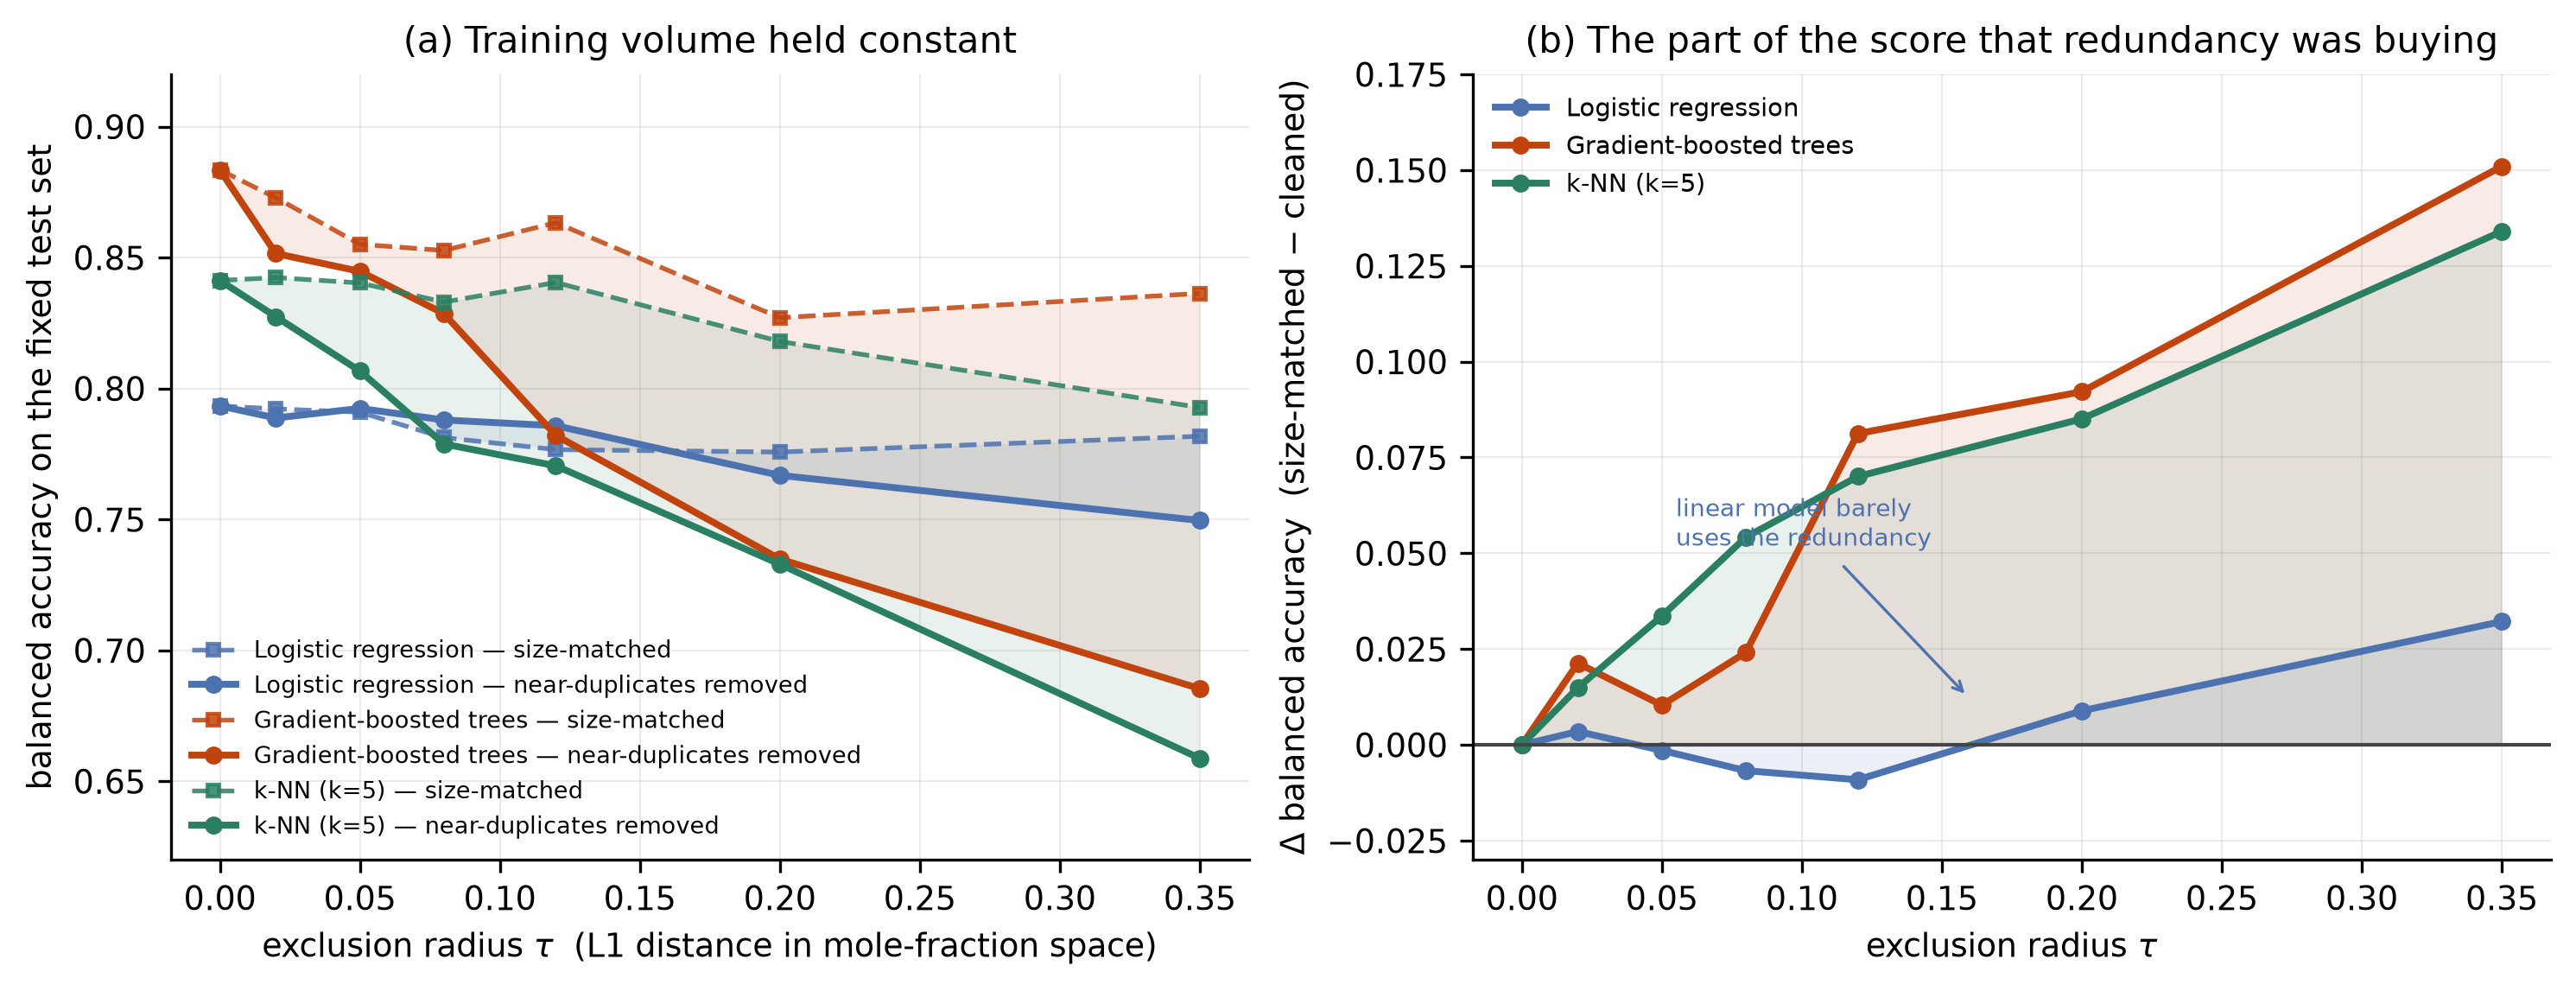
\includegraphics[width=\textwidth]{fig8_exclusion_sweep.png}
\caption{(a) Balanced accuracy on a fixed test set as the exclusion radius grows. Dashed: size-matched control. Solid: near-duplicates removed. (b) The gap between them.}
\label{fig:sweep}
\end{figure}

\begin{table}[t]
\centering
\caption{Exclusion sweep, gradient-boosted trees, means over three splits. The $\tau=0$ row is the correctness check.}
\label{tab:sweep}
\begin{tabular}{ccccc}
\toprule
$\tau$ & training size & matched control & near-duplicates removed & $\Delta$ \\
\midrule
0.00 & 882 & 0.883 & 0.883 & $0.000$ \\
0.02 & 841 & 0.873 & 0.852 & $+0.021$ \\
0.05 & 787 & 0.855 & 0.845 & $+0.010$ \\
0.08 & 720 & 0.853 & 0.829 & $+0.024$ \\
0.12 & 643 & 0.863 & 0.782 & $+0.081$ \\
0.20 & 504 & 0.827 & 0.735 & $+0.092$ \\
0.35 & 333 & 0.836 & 0.685 & $\mathbf{+0.151}$ \\
\bottomrule
\end{tabular}
\end{table}

\begin{figure}[t]
\centering
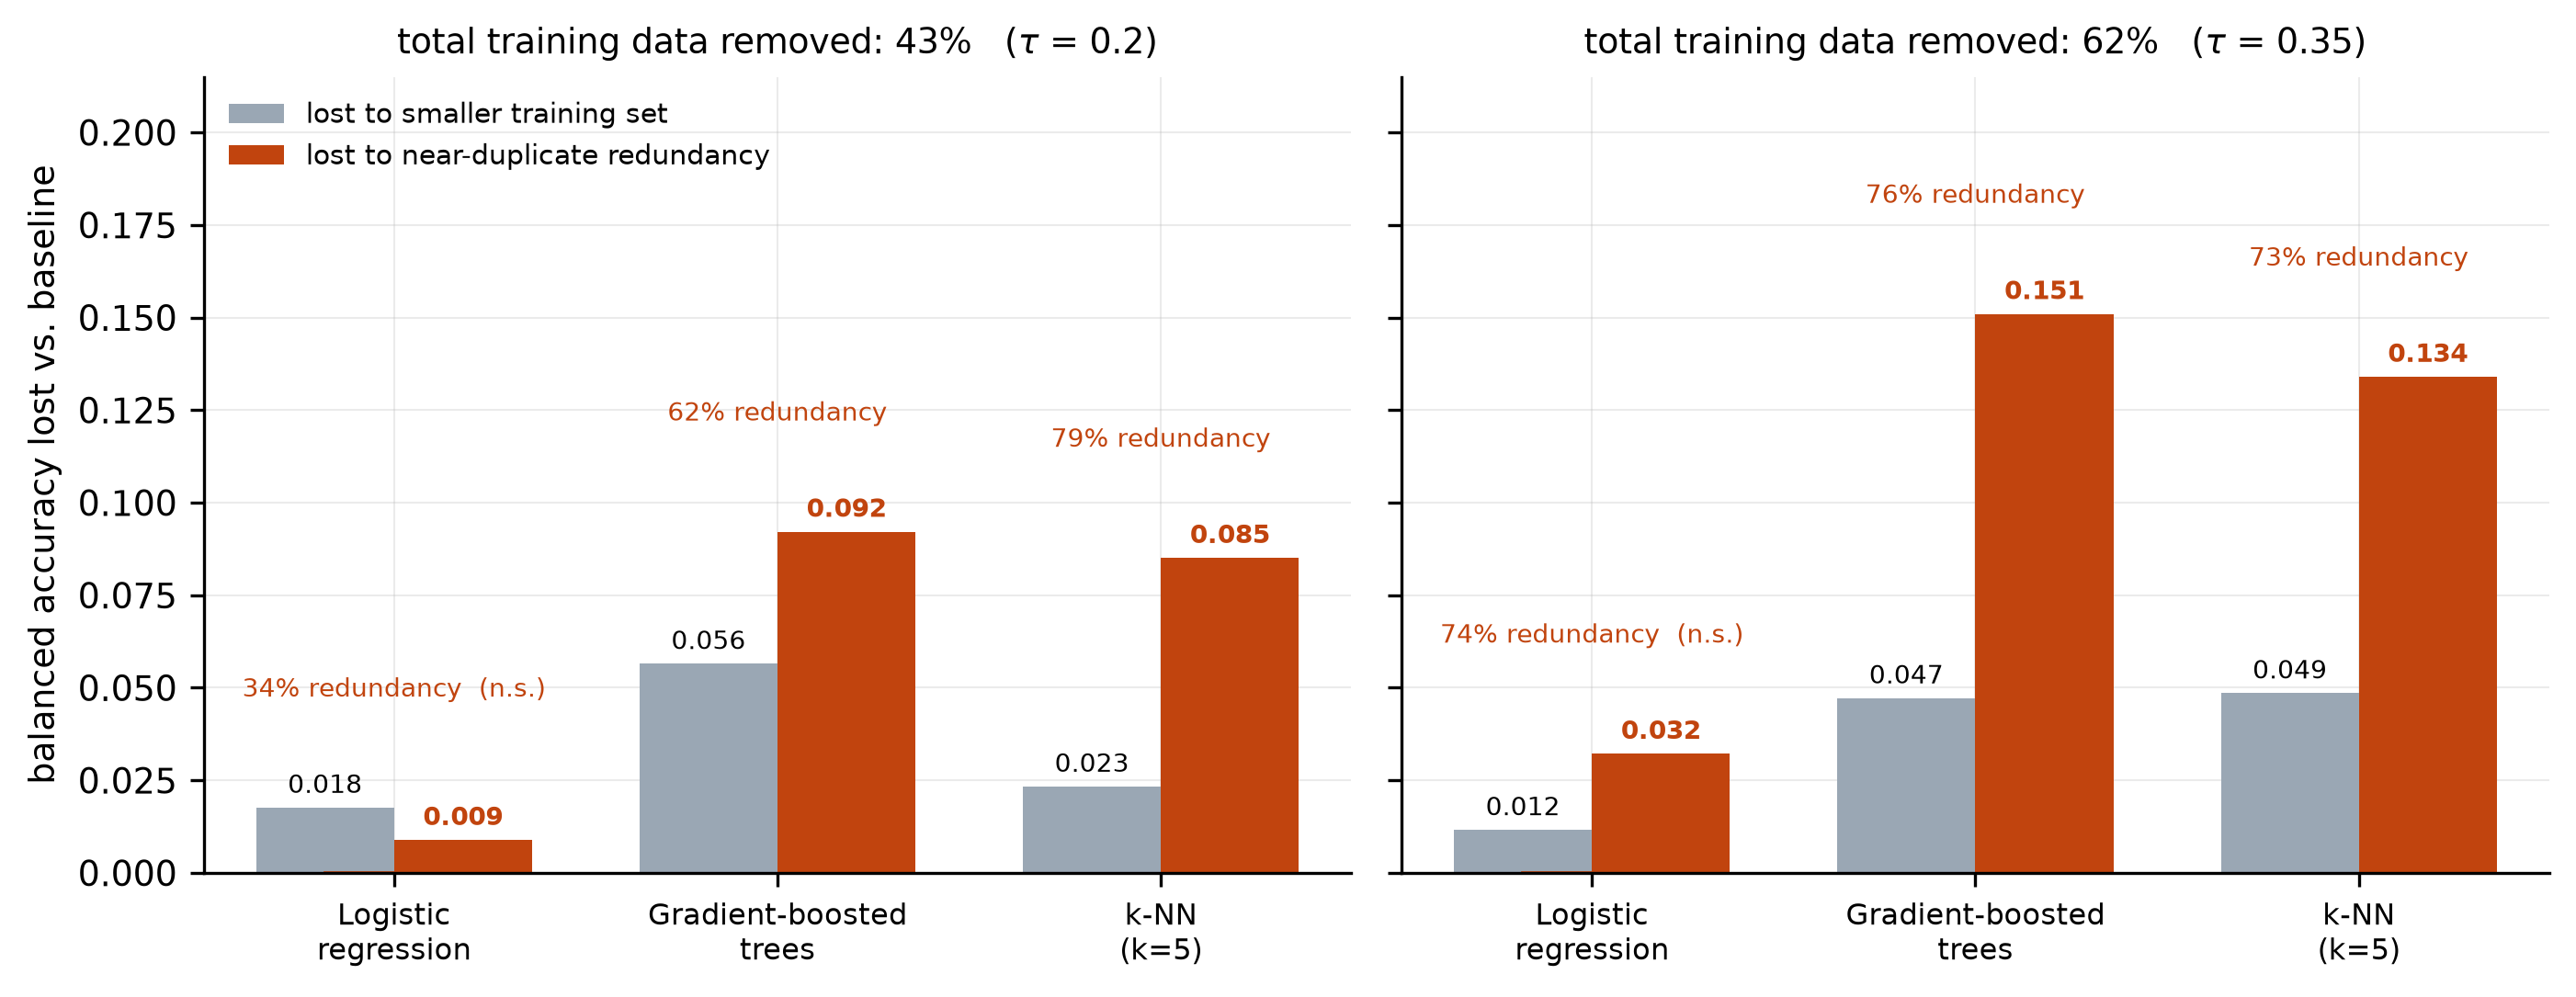
\includegraphics[width=0.92\textwidth]{fig9_variance_split.png}
\caption{How the total apparent loss splits between a smaller training set and removed redundancy.}
\label{fig:split}
\end{figure}

\begin{table}[t]
\centering
\caption{Variance decomposition at $\tau = 0.35$, where \SI{62}{\percent} of the training set has been removed.}
\label{tab:decomp}
\begin{tabular}{lcccc}
\toprule
Model & total loss & smaller training set & redundancy & redundancy share \\
\midrule
Gradient-boosted trees & 0.198 & 0.047 & \textbf{0.151} & \SI{76}{\percent} \\
$k$-NN ($k=5$)         & 0.183 & 0.049 & \textbf{0.134} & \SI{73}{\percent} \\
Logistic regression    & 0.044 & 0.012 & 0.032 & \SI{74}{\percent} (n.s.) \\
\bottomrule
\end{tabular}
\end{table}

At $\tau = 0.35$, the matched control drawn randomly to the same 333 examples still scores 0.836, barely below the 0.883 baseline, while the cleaned set scores 0.685. For the two high-capacity models, roughly three quarters of the apparent cost of a stricter evaluation protocol is redundancy, not data volume. The logistic regression result makes the story coherent: its 0.032 split is smaller than the between-split spread, so a linear model is essentially indifferent to whether near-duplicates are present.

The $\tau$-dependence is the most interesting part, and it is not what I expected going in.

\begin{itemize}
\item \textbf{Strict near-duplicates contribute almost nothing.} Removing every training alloy within 0.05 $L_1$ of a test alloy --- an \SI{11}{\percent} cut of the training set, while \SI{25.5}{\percent} of test alloys had such a neighbour (Section~\ref{sec:nn}) --- moves boosted-tree accuracy by 0.010. Deleting the ``duplicates'' is not where the fix is.
\item \textbf{The inflation lives in the middle band.} $\Delta$ rises from 0.010 at $\tau = 0.05$ to 0.081 at $\tau = 0.12$ and 0.092 at $\tau = 0.20$. The relevant redundancy is not identical compositions but \emph{same chemical system, different stoichiometry} --- alloys a model can still memorise a local answer for.
\item \textbf{It is monotone and capacity-gated.} $\Delta$ climbs steadily for boosted trees and $k$-NN; for logistic regression it oscillates around zero (mean 0.005 across $\tau \ge 0.02$, maximum 0.032 against a between-split spread of similar size).
\end{itemize}

\subsection{Mechanism: nearest-neighbour composition distance}
\label{sec:nn}

\begin{figure}[t]
\centering
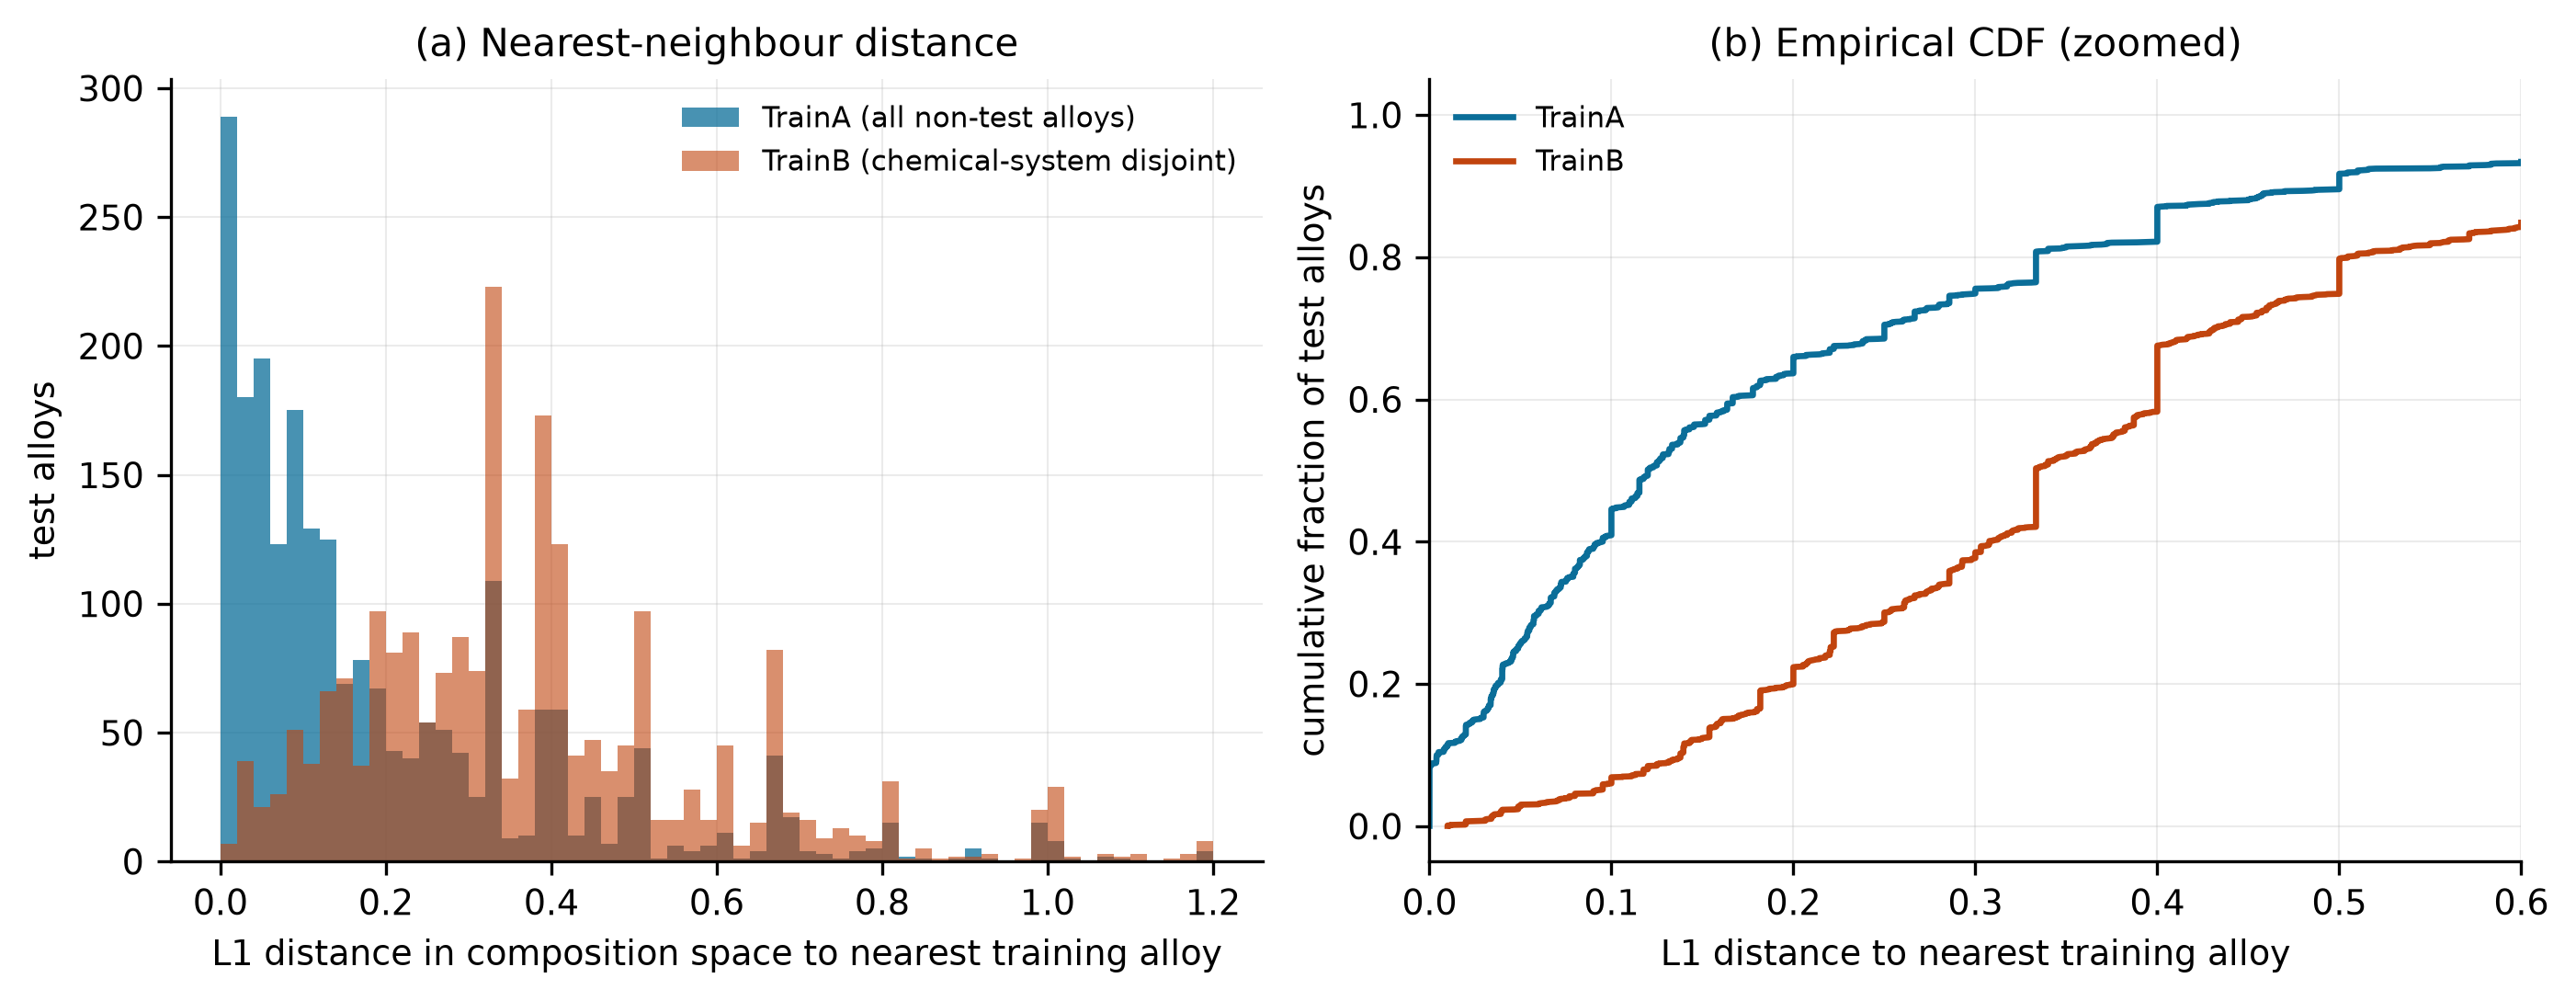
\includegraphics[width=0.78\textwidth]{fig6_neighbour_distance.png}
\caption{Distance from each test alloy to its nearest training neighbour.}
\label{fig:nn}
\end{figure}

\begin{table}[t]
\centering
\caption{Nearest-neighbour composition distance, random versus disjoint training sets.}
\label{tab:nn}
\begin{tabular}{lcc}
\toprule
Quantity & TrainA (random) & TrainB (disjoint) \\
\midrule
Median nearest-neighbour distance & 0.120 & 0.333 \\
Share below 0.05 & \textbf{\SI{25.5}{\percent}} & \SI{2.8}{\percent} \\
Share below 0.10 & \textbf{\SI{43.5}{\percent}} & \SI{6.5}{\percent} \\
\bottomrule
\end{tabular}
\end{table}

Under a random split, a quarter of the test set has an almost identical training counterpart and nearly half sits within 0.10. Under the disjoint split those numbers collapse. This is the mechanism behind everything above, and it explains why the sweep's middle band (0.10--0.20) is where the accuracy is hiding: that is where the bulk of the test set's neighbours live.

\subsection{Leave-one-element-out extrapolation}

\begin{figure}[t]
\centering
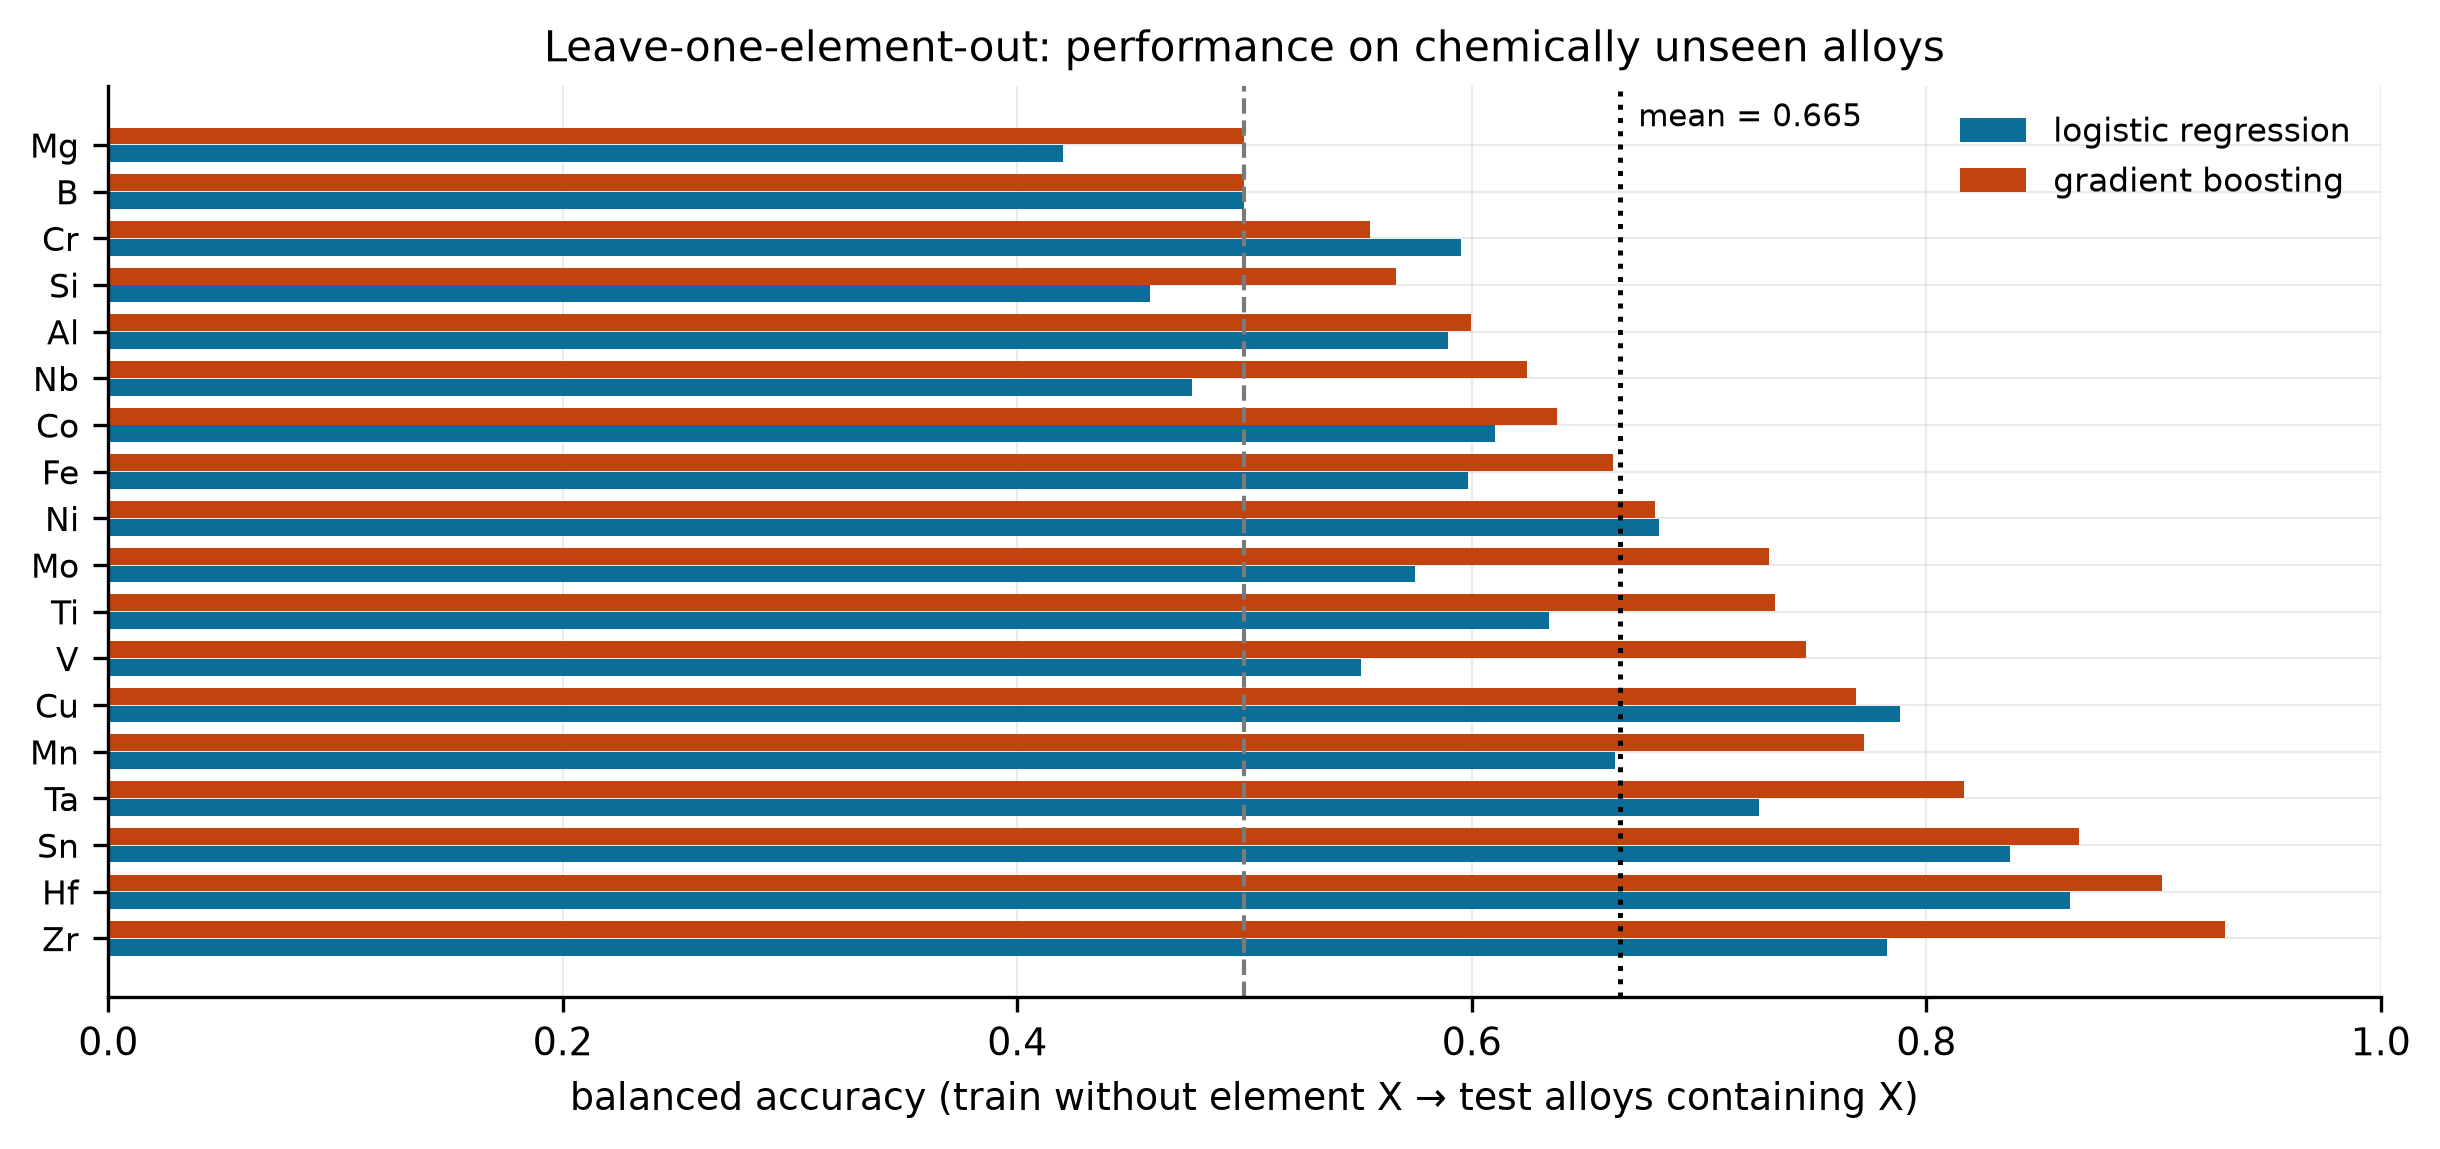
\includegraphics[width=0.78\textwidth]{fig7_loeo.png}
\caption{Balanced accuracy when a single element is held out entirely.}
\label{fig:loeo}
\end{figure}

Holding out one element at a time gives a mean balanced accuracy of \textbf{0.665} (sd 0.133, range 0.420--0.931) and mean ROC-AUC 0.776. Against the random-split figure of 0.859, that is a gap of nearly 0.2. The failure modes are chemically legible: Al (0.600) and Si (0.567) are strong intermetallic formers, and Mg (0.500) and B (0.500) have too little data to learn anything. Best extrapolation is to Zr (0.931) and Hf (0.904), chemically similar to well-represented elements.

\section{What this means}

For this dataset, and for any HEA dataset with the same ``one system, many stoichiometries'' structure:

\begin{enumerate}
\item \textbf{A random-split number is not a generalisation estimate.} For high-capacity models the overstatement here is 0.08--0.15 balanced accuracy, larger than the difference between most competing model architectures.
\item \textbf{Report at least one chemical-system-disjoint split.} It costs one extra line of code (\texttt{GroupKFold} with the element set as the group) and changes the conclusion of a paper more than most hyper-parameter searches do.
\item \textbf{Report balanced accuracy and MCC.} With a \SI{31.7}{\percent} positive rate, always predicting the majority class scores 0.683 raw accuracy, so raw accuracy flatters every model on this task.
\item \textbf{Do not bother de-duplicating exact compositions.} It is the intuitive fix and it recovers almost nothing (0.010). The redundancy that matters is structural, spread across same-system neighbours. A distance-based exclusion at $\tau \approx 0.10$--$0.20$, or an element-set split, is what actually bites.
\item \textbf{Separate the two questions.} ``Can a solid solution form'' is hard (descriptor ceiling $\approx 0.75$). ``FCC or BCC'' is easy (\SI{100}{\percent} on the decidable subset). Reporting them together hides both facts.
\item \textbf{Use leave-one-element extrapolation as a stress test.} It is cheap and it exposes which elements the model has genuinely learned versus memorised.
\end{enumerate}

The measurement protocol transfers. Any dataset where records cluster into families --- materials, bioactivity series, clinical cohorts from the same site --- can be run through the same sweep: fix the test set, vary an exclusion radius, and report how much of the headline number survives at matched training size.

\section{Limitations}

\begin{itemize}
\item \textbf{One dataset.} The magnitudes are specific to this table. The direction and the capacity dependence should transfer; the exact 0.151 should not be quoted as a universal constant.
\item \textbf{Label noise.} Labels come from aggregating literature; processing route and thermal history are not recorded. SS+IM is inherently an intermediate category and probably the largest source of irreducible error.
\item \textbf{Grouping is approximate.} ``Same element set'' is a coarse proxy for ``same chemical family'', and the exclusion sweep uses raw composition distance, which ignores chemistry. Stricter grouping would give a \emph{larger} effect, so the numbers here are lower bounds.
\item \textbf{Three model families, no capacity sweep.} Hyper-parameters were deliberately left untuned to keep protocols comparable. A proper capacity sweep would show where the transition from ``indifferent'' to ``exploiting'' happens.
\item \textbf{Three splits in the sweep.} The paired $\Delta$ at $\tau = 0.35$ is well outside the between-split spread, but the intermediate radii are not individually resolved. The monotone trend is the claim; individual small values are not.
\item \textbf{No external validation.} Nothing here was checked against new experiments; the study is entirely a re-analysis of published data.
\end{itemize}

\section{Reproducibility}

\begin{verbatim}
research/
  data/     raw workbook (read-only) + cleaned parquet/csv
  code/     hea_common.py, 00_profile.py, 01_build_dataset.py,
            02_criteria_audit.py, 03_leakage_experiment.py,
            04_figures.py, 05_report.py, 06_report_en.py,
            07_exclusion_sweep.py, 08_paper_figures.py
  out/      result JSON/CSV, all numbers quoted above
  figures/  9 figures at 300 dpi
  report/   full HTML and Markdown reports (Chinese and English)
\end{verbatim}

\begin{verbatim}
cd research/code
python 00_profile.py && python 01_build_dataset.py && python 02_criteria_audit.py
python 03_leakage_experiment.py stage1
python 03_leakage_experiment.py stage2
python 03_leakage_experiment.py merge
python 07_exclusion_sweep.py run
python 07_exclusion_sweep.py merge
python 04_figures.py && python 08_paper_figures.py
\end{verbatim}

Python 3.13 with numpy, pandas, scipy, scikit-learn, matplotlib, openpyxl, pyarrow. Every seed is fixed in the scripts. Every number in this manuscript was read at build time from the files under \texttt{out/}; none was transcribed by hand.

\section*{Declarations}

\paragraph{Use of AI tools.} This study was carried out with substantial assistance from an AI system, which ran the analysis pipeline, produced the figures and drafted the text. The AI did not generate any data; all data are third-party published measurements. The author specified the research question, reviewed the analysis, and takes responsibility for the content, including any errors. This disclosure follows current publisher policies on AI-assisted research; readers should weigh the results accordingly.

\paragraph{Data availability.} Zenodo record 6403257, DOI 10.5281/zenodo.6403257, CC-BY-4.0. The dataset was not modified.

\paragraph{Code availability.} [REPOSITORY URL --- to be filled in before submission.]

\paragraph{Competing interests.} None.

\paragraph{Funding.} None.

\begin{thebibliography}{9}

\bibitem{zenodo}
Precker, C. E., Gregores Coto, A. \& Mu\'i\~nos Land\'in, S.
\emph{Materials for Design Open Repository. High Entropy Alloys}.
Zenodo (2021). DOI 10.5281/zenodo.6403257. CC-BY-4.0.

\bibitem{zhang2008}
Zhang, Y., Zhou, Y. J., Lin, J. P., Chen, G. L. \& Liaw, P. K.
Solid-solution phase formation rules for multi-component alloys.
\emph{Advanced Engineering Materials} \textbf{10}, 534--538 (2008).

\bibitem{yang}
Yang, X. \& Zhang, Y.
Prediction of high-entropy stabilized solid-solution in multi-component alloys.
\emph{Materials Chemistry and Physics} \textbf{132}, 233--238 (2012).

\bibitem{guo2011}
Guo, S. \& Liu, C. T.
Phase stability in high entropy alloys: formation of solid-solution phase or amorphous phase.
\emph{Progress in Natural Science: Materials International} \textbf{21}, 433--446 (2011).

\bibitem{guojap}
Guo, S., Ng, C., Lu, J. \& Liu, C. T.
Effect of valence electron concentration on stability of fcc or bcc phase in high entropy alloys.
\emph{Journal of Applied Physics} \textbf{109}, 103505 (2011).

\bibitem{datasail}
Joachimiak, M. P., Nielsen, J. S. \& Winther, O.
Data splitting to avoid information leakage with DataSAIL.
\emph{Nature Communications} \textbf{16} (2025).

\bibitem{kapoor}
Kapoor, S. \& Narayanan, A.
Leakage and the reproducibility crisis in machine-learning-based science.
\emph{Patterns} \textbf{4}, 100804 (2023).

\end{thebibliography}

\vspace{1em}
\noindent\small\itshape
The dataset belongs to its original authors; nothing in this manuscript is a criticism of any specific published work. The claim is narrow: on this dataset, under this protocol, this much of the reported accuracy is redundancy.

\end{document}
